
%use square brackets as golang text templating delimiters
\documentclass{article}
\usepackage{graphicx}
\usepackage[margin=1in]{geometry}

\graphicspath{ {images/} }
\begin{document}
\title{Текущее состояние (протокол обмена данными S7)  \\ \large All, All, All, All, All, All, All, All  }
\date{Tue Jun 21 11:07:33 MSK 2022\\to\\Tue Jun 21 11:12:33 MSK 2022}
\maketitle
\begin{center}
\par
\vspace{0.5cm}

\includegraphics[width=\textwidth]{image15}
\par
\vspace{0.5cm}
\par
\vspace{0.5cm}
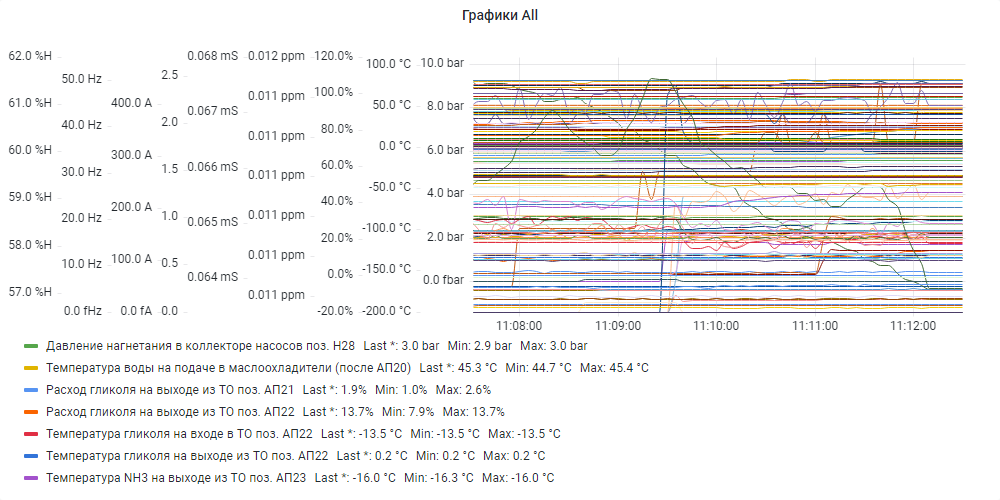
\includegraphics[width=\textwidth]{image12}
\par
\vspace{0.5cm}
\par
\vspace{0.5cm}

\includegraphics[width=\textwidth]{image154}
\par
\vspace{0.5cm}
\par
\vspace{0.5cm}
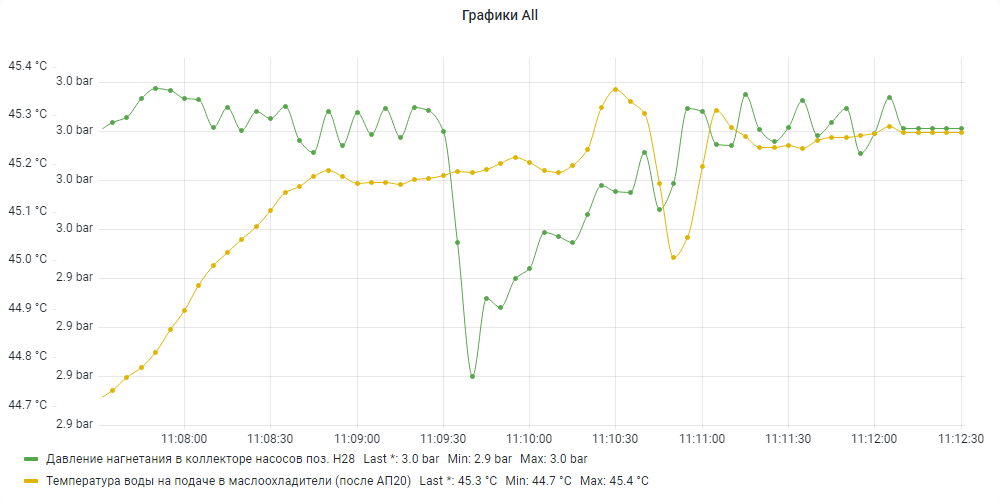
\includegraphics[width=\textwidth]{image156}
\par
\vspace{0.5cm}


\end{center}
\end{document}
